As a first step, we are going to take a look at how KeePass and FIDO2
work individually. After that, we can examine the options of combining them.

\section{KeePass password manager}\label{section:keepass-password-manager}

KeePass is a free open source password manager licensed under GNU \glsxtrfull{gpl}.
It stores passwords, and all associated data, such as usernames, URLs, notes, etc. in a single \emph{\gls{database}} file,
which is encrypted using a \emph{\gls{master key}}. The supported encryption algorithms include \glsxtrfull{aes} and ChaCha20~\cite{keepass:home}.

The \gls{master key} is based on one or more \emph{\glspl{key source}}:

\begin{itemize}
	\item a master password,
	\item a key file, which can be any file, located anywhere on the system or external storage,
	\item a windows user account, in which case \glsxtrfull{dpapi} is used.
\end{itemize}

Any of these sources may be used on its own or be combined with others~\cite{keepass:keys}.

KeePass is written primarily for the Windows operating system and can be run on other systems
via Mono or Wine~\cite{keepass:setup}. There are many unofficial KeePass ports to other platforms, including
Android, iOS, Linux, and OS X. These ports usually aim to implement the same database format,
i.e., they might be able to use a database created by the official version, but the overall
set of features and implementation details may differ considerably~\cite{keepass:download}. This work will focus only on the official version
but will try to preserve database compatibility with other versions, if possible.

\subsection{KeePass plugin system}\label{subsec:keepass-plugin-system}

KeePass offers an extensive plugin system, and a list of known plugins is maintained at its official website~\cite{keepass:plugins}.
Looking at the categories of available plugins provides a good overview of what the plugin system allows:

\begin{itemize}
	\item I/O \& Synchronization \textendash\ loading or synchronizing a database from a remote storage provider,
	\item Integration \& Transfer \textendash\ improving integration with other applications for easier transfer of credentials,
	\item Cryptography \& Key Providers \textendash\ adding new encryption methods or key sources,
	\item Import \& Export \textendash\ interoperability with other systems.
\end{itemize}

This is, of course, not an extensive list of the plugins system's capabilities.

The plugins are authored in C\#, using the .NET Framework, and need to derive from a base KeePass plugin class,
which defines hooks for KeePass lifecycle events as seen in \autoref{fig:minimal-keepass-plugin}~\cite{keepass:plugin-development}.

\begin{figure}[H]
	\begin{minipage}[]{\linewidth}
		\begin{minted}{csharp}
			using KeePass.Plugins;

			namespace SimplePlugin
			{
				public sealed class SimplePluginExt : Plugin
				{
					private IPluginHost m_host = null;

					public override bool Initialize(IPluginHost host)
					{
						if (host == null) return false;
						m_host = host;
						return true;
					}
				}
			}
		\end{minted}
	\end{minipage}

	\caption[A minimal KeePass plugin]
	{A minimal KeePass Plugin~\protect\cite{keepass:plugin-development}}
	\label{fig:minimal-keepass-plugin}
\end{figure}

The \mintinline{csharp}{IPluginHost} interface provides access to most of KeePass's internals. Several sample plugins
are available, demonstrating the most common use-cases, such as:

\begin{itemize}
	\item creating a custom password generator algorithm,
	\item creating a custom encryption algorithm,
	\item customizing the UI elements~\cite{keepass:plugins}.
\end{itemize}

The plugins can be distributed as a \glsxtrshort{dll} file, a PLGX\footnote{\Glsdesc{plgx}.} file, or both~\cite{keepass:plugin-development}.
The advantages and disadvantages of these options are summarized in~\autoref{tab:dll-vs-plgx}.

\begin{table}[H]
	\caption[Comparison of DLL and PLGX plugin format]
	{Comparison of DLL and PLGX plugin format~\protect\cite{keepass:plugin-development}}
	\label{tab:dll-vs-plgx}

	\begin{tabular}{|c|c|c|}
		\hline
		& DLL                                       & PLGX                              \\
		\hline
		\hline
		Compatibility check                         & No - weak only    & Yes - strong  \\
		\hline
		Compatibility with custom builds (Linux)    & Partial           & Yes           \\
		\hline
		Authenticode signing support                & Yes               & No            \\
		\hline
		No compilation on the user's system         & Yes               & No            \\
		\hline
		No plugin cache                             & Yes               & No            \\
		\hline
	\end{tabular}
\end{table}

\subsection{KeePass key providers}\label{subsec:keepass-key-providers}

In the previous section, we found there is a category of plugins called key providers,
which allow implementing alternative ways of unlocking the database.
Key providers derive from the \mintinline{csharp}{KeePassLib.Keys.KeyProvider} class
and register themselves in the key provider pool via the \mintinline{csharp}{Add} method of the \mintinline{csharp}{KeyProviderPool} class provided by \mintinline{csharp}{IPluginHost} interface~\cite{keepass:key-provider-development}, as seen in \autoref{fig:minimal-key-provider}.
This design follows a strategy pattern\footnote{A behavioral software design pattern that allows us to define a family of algorithms, make them interchangeable, and select a specific one at runtime~\cite{design-patterns}.}
that allows users to select which of the registered providers will be used at database creation time.

In this section, we will briefly examine some of the existing implementations.
This is not meant to be an extensive list of key providers nor a detailed examination of their implementation details,
but rather a small selection of well-documented, actively developed, and used\footnote{
	The KeePass website lists several plugins implementing support for RSA certificates, for example,
	which might be conceptually similar to our plugin, but after a short inspection, we found that they are either no longer available~\cite{keepass:plugin:multi-cert, keepass:plugin:rsa-cert},
	or not actively developed and used~\cite{keepass:plugin:cert-key} (judging by a lack of author and user activity, and little or no documentation).
} open source implementations that we can use
as a reference later when discussing our own implementation challenges.

KeePassQuickUnlock is a plugin that allows reopening the database without a full master password. It only works if the database is closed
and later reopened, but KeePass stayed running\textemdash in that case, the full master key is kept in memory, and only
a few characters of the master password are required to confirm the unlock~\cite{keepass:plugin:quick-unlock}.

Similarly to KeePassQuickUnlock, KeePassWinHello is intended for quickly unlocking the database\textemdash after its first regular unlock\textemdash using \gls{Windows Hello}\footnote{\Glsdesc{Windows Hello}.}
technology. By default, the plugin holds an encrypted master key in memory and removes it when KeePass is closed.
In order to be able to unlock the database via Windows Hello in between KeePass launches, it
may be configured to store the key in the \gls{Windows Credential Manager}\footnote{\Glsdesc{Windows Credential Manager}.}~\cite{keepass:plugin:win-hello}.

\begin{figure}[H]
	\begin{minted}{csharp}
		namespace KeyProviderTest
		{
			public sealed class KeyProviderTestExt : Plugin
			{
				private IPluginHost m_host = null;
				private SampleKeyProvider m_prov = new SampleKeyProvider();

				public override bool Initialize(IPluginHost host)
				{
					m_host = host;
					m_host.KeyProviderPool.Add(m_prov);
					return true;
				}

				public override void Terminate()
				{
					m_host.KeyProviderPool.Remove(m_prov);
				}
			}

			public sealed class SampleKeyProvider : KeyProvider
			{
				public override string Name
				{
					get { return "Sample Key Provider"; }
				}

				public override byte[] GetKey(KeyProviderQueryContext ctx)
				{
					// Return a sample key. In a real key provider plugin, the key
					// would be retrieved from smart card, USB device, ...
					return new byte[]{ 2, 3, 5, 7, 11, 13 };
				}
			}
		}
	\end{minted}

	\caption[A minimal KeePass key provider]
	{A minimal KeePass key provider~\protect\cite{keepass:key-provider-development}}
	\label{fig:minimal-key-provider}
\end{figure}

\section{FIDO2}\label{sec:fido2}

FIDO2 is a term used to refer to several related specifications, which together,
"enable users to leverage common devices to easily authenticate to online services in both mobile and desktop environments"~\cite{fido:fido2}.
The specifications are the \glsxtrfull{webauthn} specification by \glsxtrfull{w3c}
and the \glsxtrfull{ctap} specification by FIDO Alliance\footnote{\Glsdesc{FIDO Alliance}.}.

The security model of FIDO2 is based on public-key cryptography,
and three main entities:

\begin{itemize}
	\item a \emph{\glsxtrfull{RP}}\ \textendash\ \glsdesc{rp}, and which stores the public key,
	\item an \emph{\gls{authenticator}} \textendash\ \glsdesc{authenticator},
	\item a \emph{\gls{client}} \textendash\ \glsdesc{client}~\cite{fido:webautn}.
\end{itemize}

For each \gls{rp}, a separate public and private key pair is used, instead of a regular
password.

The \gls{authenticator} may be either a separate hardware device (a \emph{\gls{roaming authenticator}}),
or a platform implementation (a \emph{\gls{platform authenticator}}).
The main difference is that while a \gls{roaming authenticator} is transferable between
\emph{\glspl{client device}}\footnote{\Glsdesc{client device}.},
a \gls{platform authenticator} is bound to a specific \gls{client device}.
A \gls{platform authenticator} may still use specialized hardware, e.g., a \glsxtrfull{tpm}\footnote{\Glsdesc{TPM}.}
to provide sufficient security~\cite{fido:webautn}.

Note that authenticators are often also referred to as "security keys". We will restrain
from using this term in this work to avoid confusion with frequently mentioned encryption keys.

\begin{figure}[H]
	\centering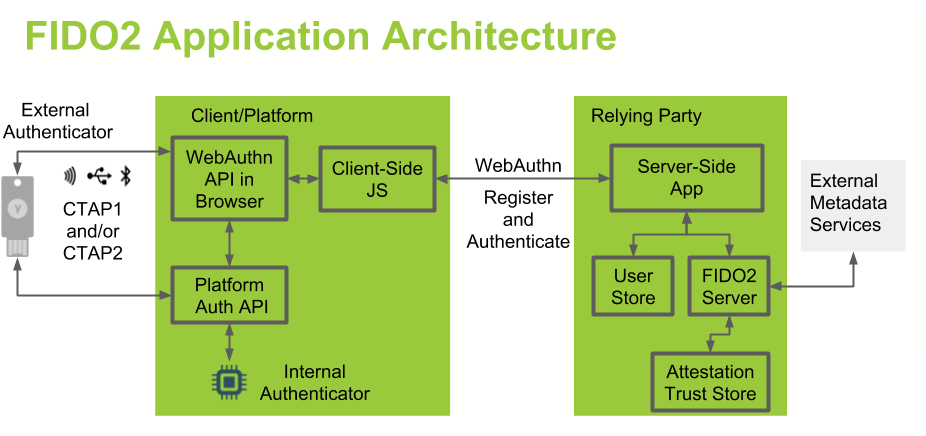
\includegraphics[width=\textwidth]{images/fido2-app-architecture}

	\caption[FIDO2 architecture]
	{FIDO2 architecture~\protect\cite{yubico:webauthn}}
	\label{fig:fido2-architecture}
\end{figure}

The FIDO Alliance summarizes the key aspects of FIDO2 as~\cite{fido:fido2}:

\begin{enumerate}
	\item \textbf{Security} \textendash\ FIDO2 cryptographic login credentials\footnote{
			The term "credential" is not well-defined by the specification, but generally means the private key
			and its associated metadata stored by the authenticator, such as information about the user account or relying party.
		} are unique across every website, never leave the user’s device, and are never stored on a server.
		This eliminates the risks of phishing, all forms of password theft, and replay attacks.
	\item \textbf{Privacy} \textendash\ Because FIDO cryptographic keys are unique for each internet site, they cannot be used to track users across sites.
	\item \textbf{Convenience} \textendash\ Users unlock cryptographic login credentials with simple
		built-in methods such as fingerprint readers or cameras on their devices, or by leveraging easy-to-use FIDO security keys.
	\item \textbf{Scalability} \textendash\ Websites can enable FIDO2 through a simple JavaScript API call that is supported across leading browsers and platforms.
\end{enumerate}\medskip

\subsection{\glsentryfull{webauthn}}\label{subsec:webauthn}

\glsxtrshort{webauthn} is the specification that covers interactions between clients and relying parties
(typically, but not necessarily, web browsers and web applications). The main interactions are
\mintinline{csharp}{Create} and \mintinline{csharp}{Get}, which serve to create new credentials and to
authenticate using existing ones.

\mintinline{csharp}{Create} can be loosely described as~\cite{fido:webautn}:

\begin{enumerate}
	\item The \gls{rp} (optionally) collects user data, sets credential creation options, and initiates the create process with the \gls{client}.
	\item The \gls{client} forwards the request to the authenticator, along with information about the \gls{rp}.
	\item The \gls{authenticator} generates a new credential and returns the public key along with additional metadata to the \gls{client}.
	\item The \gls{client} forwards the key and metadata to the \gls{rp}.
\end{enumerate}

There are two creation options that are especially important in this process, \mintinline{csharp}{userVerification} and \mintinline{csharp}{requireResidentKey},
which specify whether \gls{user verification} is required, preferred, or discouraged, and whether a \gls{resident credential} is requested.

\Gls{user verification} is \glsdesc{user verification}~\cite{fido:webautn}. In other words, this is the element that prevents
unauthorized use of the authenticator by people other than its owner who have physical access to it.
This protection is optional and can be enforced by the \gls{rp}. When enabled, it takes place
before step three.

\Gls{resident credential} is \glsdesc{resident credential}. This definition immediately raises a question:
where else could the private key be stored? The answer is that this is not specified\textemdash the authenticator
is responsible for protecting the key, but not for its physical storage. This allows implementing schemes
that offload the storage to an external system so that the number of stored keys is not limited by the authenticator's
internal memory. For example, Yubico\footnote{A member of the FIDO Alliance and a vendor of YubiKey authenticators.} uses the following process for handling non-resident keys~\cite{yubico:key-generation}:

\begin{quoting}
	During credential registration, a new key pair is randomly generated by the YubiKey, unique to the new credential.
	The private key, along with some metadata about the credential, is encrypted using authenticated encryption with
	a master key. This master key is unique per YubiKey, generated by the device itself upon first startup,
	and never leaves the YubiKey in any form [\ldots]

	The encrypted (and authenticated) data then forms the 64-byte key handle, which is sent to the server as part of
	the registration flow, to be stored by the RP for later [\ldots]

	For authentication, the RP returns the key handle to the YubiKey. Here it is decrypted to re-form the private key
	which is needed to sign the challenge to complete the authentication.
\end{quoting}

The resident credential does not necessarily provide better security, but it comes with one significant advantage
that allows simplifying the authentication process. First, let us examine how the \mintinline{csharp}{Get} operation
works with non-resident credentials~\cite{fido:webautn}:

\begin{enumerate}
	\item The \gls{rp} asks the user for a username or another identifier of the account.
	\item Based on the username, it finds all public keys and their metadata that it previously stored.
	\item The \gls{rp} generates a \emph{challenge}, \glsdesc{challenge}.
	\item The \gls{rp} initiates the get process with the client and sends it the information about public keys and the challenge.
	\item The client forwards this request to the authenticator.
	\item The authenticator performs user verification if requested.
	\item The authenticator looks up the private keys corresponding to the public keys provided by the \gls{rp}, signs the challenge using each of these keys, and returns the result to the client.
	\item The client forwards the signatures and metadata to the \gls{rp}.
\end{enumerate}

The resident credentials allow skipping the first two steps, i.e., the user does not
need to provide any account information. The authenticator looks up all credentials
associated with the \gls{rp}. If more than one exists, either the authenticator or
the client may present a list of all found credentials and let the user choose which
one should be used. If there is only one matching credential, no user input is needed.

\subsection{\glsentryfull{ctap}}\label{subsec:ctap}

This specification describes the communication between clients and authenticators,
and exact steps how authenticators handle the individual commands. The commands
are closely tied to those already described in \glsxtrshort{webauthn} so it is enough to
say that the \mintinline{csharp}{Create} operation from \glsxtrshort{webauthn} corresponds with
the \mintinline{csharp}{authenticatorMakeCredential} command, and the \mintinline{csharp}{Get} operation
is based on \mintinline{csharp}{authenticatorGetAssertion}. We may reference this specification
in later sections for specific details if they turn out to be important for this work.

\subsection{\glsentryfull{u2f}}\label{subsec:u2f}

U2F is an open standard for two-factor authentication, which can be seen as a predecessor to
FIDO2. Unlike FIDO2, it is already supported by many\footnote{The Works with YubiKey Catalog~\cite{yubico:works-with-u2f} lists tens of large-scale services, such as Dropbox, Gmail, Facebook, or Twitter. It is not a complete list as services do not need to register with Yubico in order to use U2F.}
services, and all FIDO2 devices are backward-compatible with
existing U2F implementations~\cite{yubico:u2f}. We will not directly utilize the \glsxtrshort{u2f} protocol in this work but consider it
important to note that since FIDO2 authenticators support \glsxtrshort{u2f} as well, it can be used as an addition to passwords
for services that implement U2F but not FIDO2.

\subsection{A note on terminology}\label{subsec:a-note-on-terminology}

Because FIDO2 supports various authentications flows, e.g., it can be used as:

\begin{itemize}
	\item a password replacement,
	\item a second factor, in addition to a regular username and password,
	\item a password and a username replacement, in case of a resident credential,
\end{itemize}

and because it is also backward-compatible with U2F, it is often not clear which of these flows
a specific implementation or service supports. The term FIDO2, when used in this work, always refers
to a scenario where the authenticator is used as a primary factor (a replacement for the password).
For scenarios where the authenticator is used as an additional factor, we use the term \glsxtrshort{u2f}.
